	\documentclass[11pt]{article}
	
	\title{Homework 1 - DM CS6220}
	\author{Nakul Camasamudram}
	\usepackage{amsmath,amsfonts,amsthm} % Math packages
	\usepackage{mathtools}
	\usepackage{adjustbox}
	\usepackage{soul}
	%----------------------------------------------------------------------------------------
	%	TITLE SECTION
	%----------------------------------------------------------------------------------------
	
	\newcommand{\horrule}[1]{\rule{\linewidth}{#1}} 
	
	\title{	
	\normalfont \normalsize 
	\textsc{Northeastern University, Data Mining Techniques - CS6220 Fall 2017} \\
	 % Your university, school and/or department name(s)
	\horrule{0.5pt} \\[0.4cm] % Thin top horizontal rule
	\huge Solutions to Homework 2, Part 3 \\ % The assignment title
	\horrule{2pt} \\[0.5cm] % Thick bottom horizontal rule
	}
	\author{Nakul Camasamudram} % Your name
	\date{\normalsize\today} % Today's date or a custom date
	\begin{document}
	
	\maketitle % Print the title
	\newpage
	
%----------------------------------------------------------------------------------------
	%	PROBLEM 3
	%----------------------------------------------------------------------------------------
	
\section*{3 Evaluation}

\subsection*{3.1 Cophenetic Correlation Coefficient}
\textbf{Solution:}\\
Table 8.7 from TSK: \\
\begin{center}
	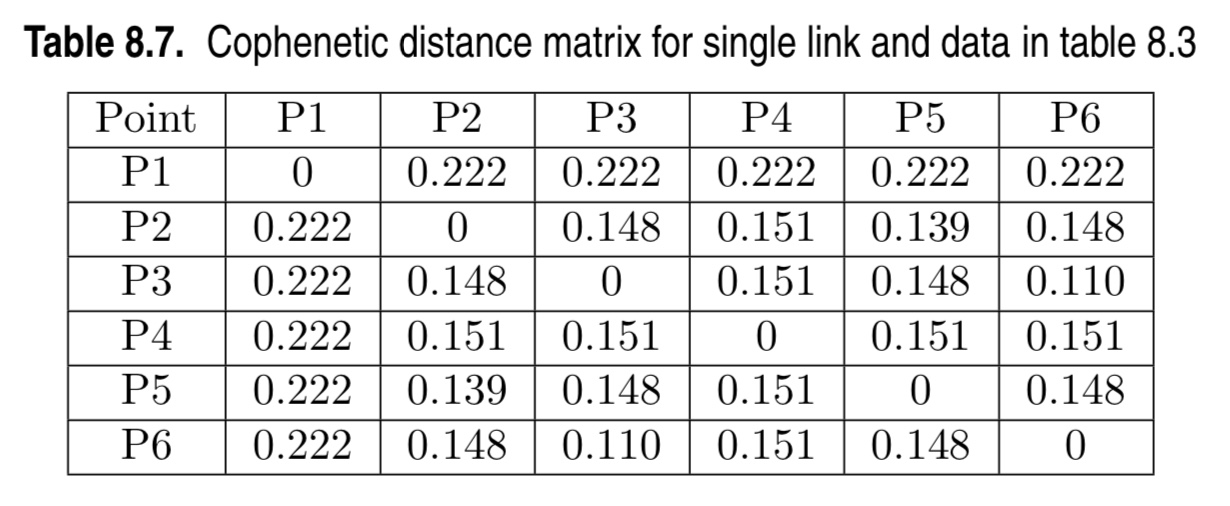
\includegraphics[scale=0.2]{table_8_7.jpeg}
\end{center}

\underline{a.}
The cophenetic distance between two clusters is the smallest distance between the two clusters when they were initially merged together.

\begin{itemize}
	\item Clusters 3 and 6 were the first to be merged in and when they were, the distance between them was 0.11
	\item Clusters 2 and 5 were merged together next and the distance between them when they were merged was 0.139
	\item and similarly for P3/P5 and P2/P6
\end{itemize}

\underline{b.}

The cophenetic correlation can be computed as follows

\begin{center}
	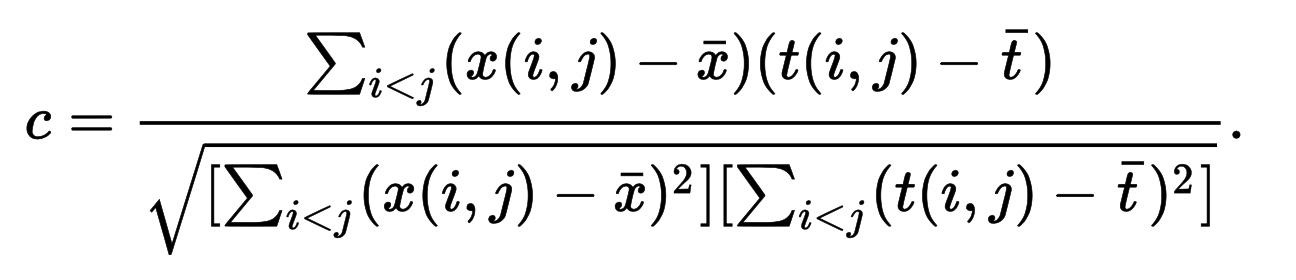
\includegraphics[scale=0.2]{cophenetic_equation.jpeg}
\end{center}

\begin{itemize}
	\item $x(i, j)$ = $| X_i - X_j |$, the ordinary Euclidean distance between the $i^{th}$ and $j^{th}$ observations
	\item $t(i, j)$ = the cophenetic distance between the points $T_i$ and $T_j$
\end{itemize}

\underline{Computation:}
\begin{center}
	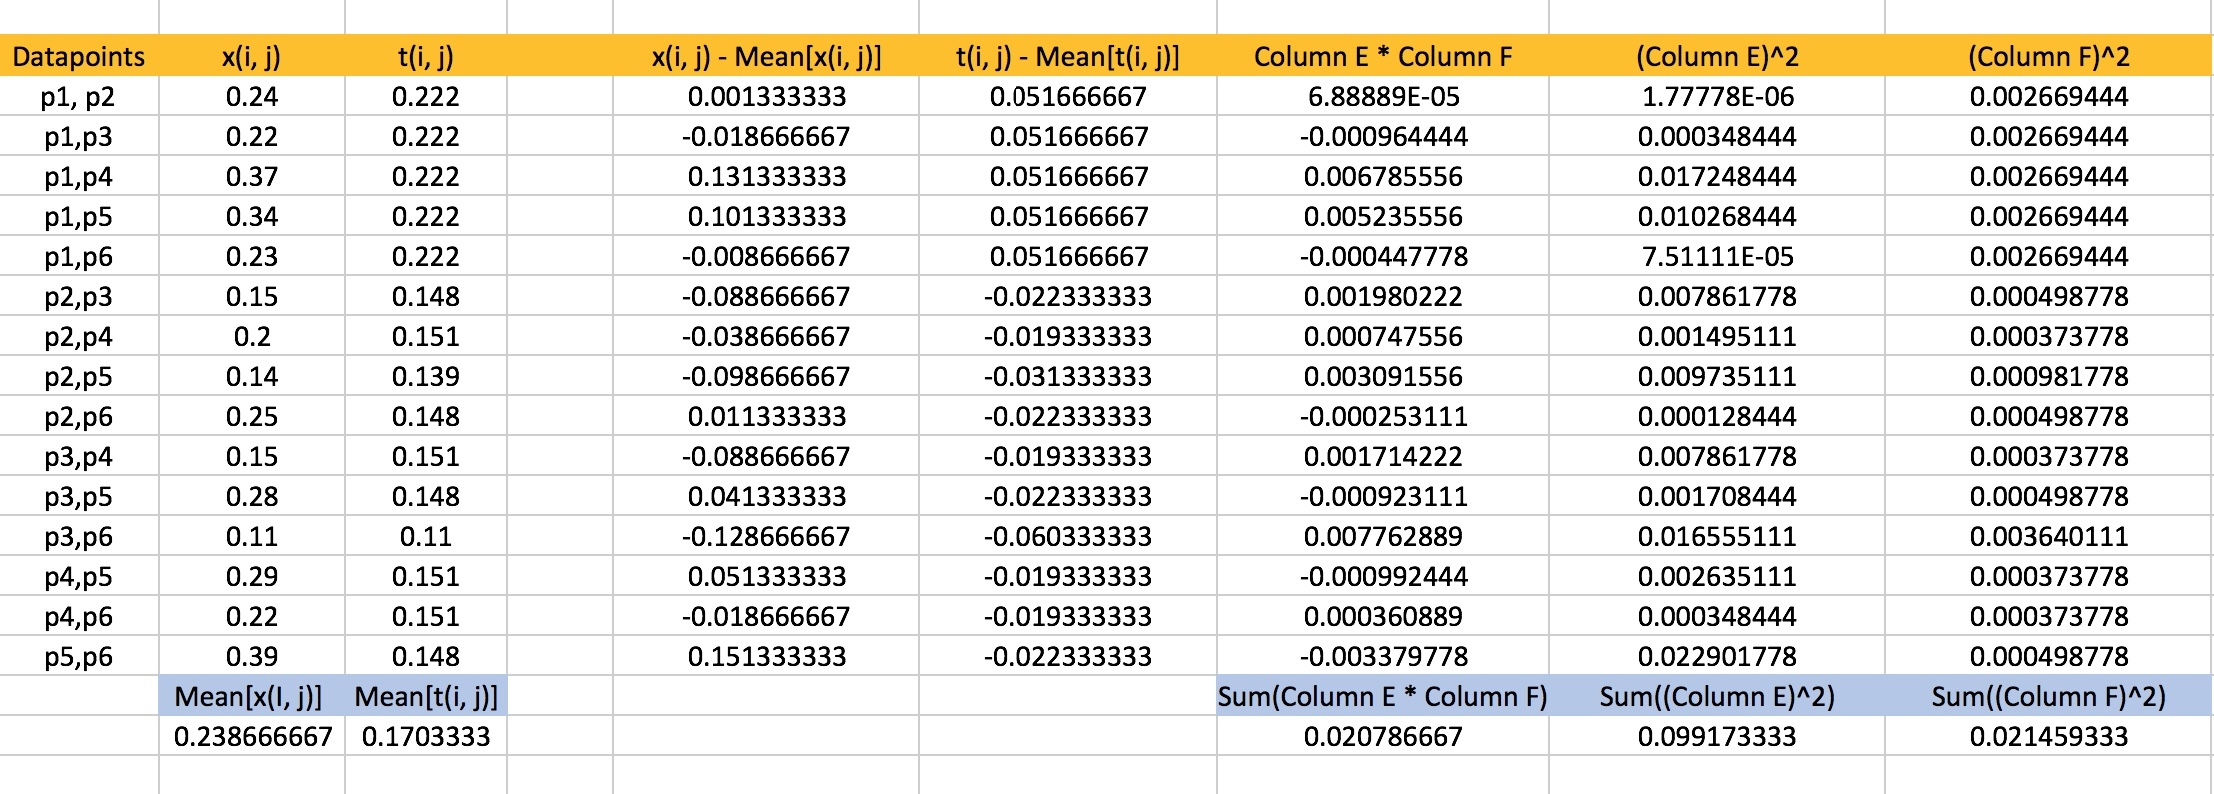
\includegraphics[scale=0.2]{cophenetic_excel}
\end{center}

Using the above equation and computations from the table,

\begin{align*}
	c &= \frac{Sum(Column E * Column F)}{\sqrt{Sum((Column E)^2) \cdot Sum((Column F)^2)}} \\
	&= \frac{0.020786667}{\sqrt{0.099173333 \times 0.021459333}} \\
	&= 0.450587616
\end{align*}


\subsection*{3.2 Purity}
\textbf{Solution:}\\

Table 8.9 from TSK: \\
\begin{center}
	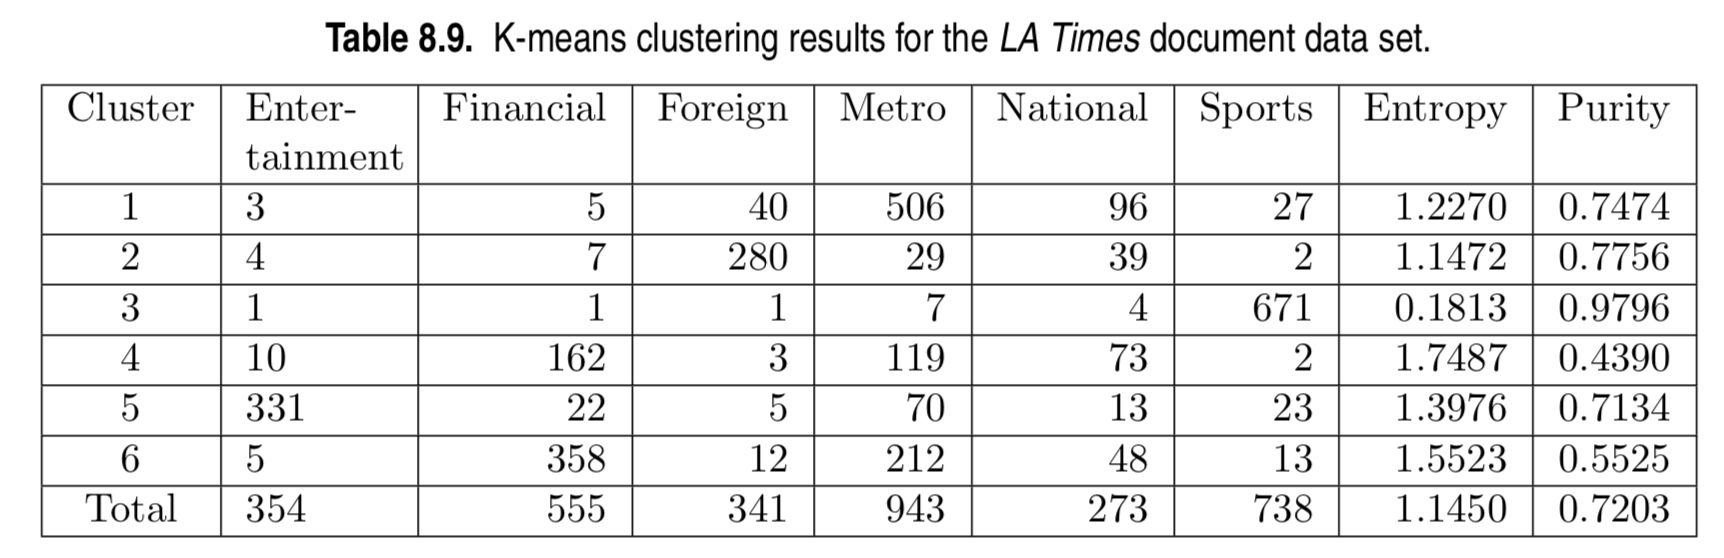
\includegraphics[scale=0.2]{table_8_9.jpeg}
\end{center}

\underline{a. Calculation:}
Let $p_i$ be the purity of the $i^{th}$ cluster, $m_i$ be the number of objects in the $i_{th}$ cluster and $m_{ij}$ be the number of objects of class $j$ that under cluster $i$.

\begin{itemize}
	\item $p_1 = \frac{1}{m_1} \cdot max_{j}(m_{1j}) = \frac{1}{677} \cdot 506 = 0.7474$
	\item $p_2 = \frac{1}{m_2} \cdot max_{j}(m_{2j}) = \frac{1}{361} \cdot 280 = 0.7756$
	\item $p_3 = \frac{1}{m_3} \cdot max_{j}(m_{3j}) = \frac{1}{685} \cdot 671 = 0.9796$
	\item $p_4 = \frac{1}{m_4} \cdot max_{j}(m_{4j}) = \frac{1}{369} \cdot 162 = 0.4390$
	\item $p_5 = \frac{1}{m_5} \cdot max_{j}(m_{5j}) = \frac{1}{464} \cdot 331 = 0.7134$
	\item $p_6 = \frac{1}{m_6} \cdot max_{j}(m_{6j}) = \frac{1}{648} \cdot 358 = 0.5525$
\end{itemize}	

Overall purity of the clustering = $\sum^{6}_{i = 1} \frac{m_i}{m} \cdot p_i = \frac{1}{[354 + 555 + 341 + 943 + 273 + 738]} \cdot [506 + 280 + 671 + 162 + 331 + 358] = 0.7203$
\\

\underline{b. }
Purity is a measure of the extent to which each cluster contains only objects from a single class. So, ideally, the overall purity of the clustering should be $1$. In the above case, since it is $0.72034$, the clustering is good.

By this metric, Cluster 3 is particularly good as it contains objects almost entirely from the "Sports" class.
	
	
	
\end{document}